%%%%%%%%%%%%%%%%%%%%%%%%%%%%%%%%%%%%%%%%%%%%%%%%%%%%%%%%%%%%%%%%%%%%
% Authors: A. Herrera-Poyatos, F. Herrera
% Tittle: Algoritmo memético equilibrado con diversificación voraz
% 							 CAEPIA 2015
%%%%%%%%%%%%%%%%%%%%%%%%%%%%%%%%%%%%%%%%%%%%%%%%%%%%%%%%%%%%%%%%%%%%

\section{Motivación}

{
	% Set the headline 
	\setbeamertemplate{headline}{
		\begin{beamercolorbox}[sep=4pt]{title} 
			\usebeamerfont{title} Motivación: Problema de la diversidad de la población 
		\end{beamercolorbox}
	}

	% Remove space between formulas and text.
	\setlength{\belowdisplayskip}{1pt} \setlength{\belowdisplayshortskip}{0pt}
	\setlength{\abovedisplayskip}{1pt} \setlength{\abovedisplayshortskip}{0pt}	
	
	\begin{frame}{}

		% Font size
		\fontsize{9}{10}\selectfont

		\begin{definition}
			La \textbf{diversidad de la población} se define como la media de las distancias entre todas las parejas de cromosomas.
			\begin{gather*}
				D(P) = \frac{\sum_{s,s' \in P} d(s,s')}{n(n-1)}
			\end{gather*}
		\end{definition}

		\begin{columns}[c]
			
			\column{.6\textwidth}

				\centering 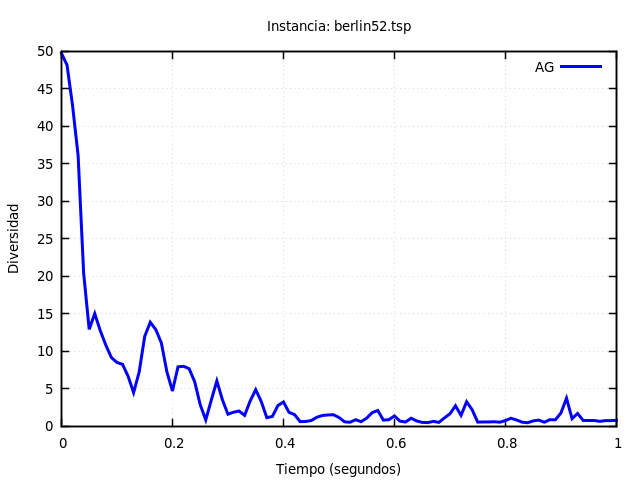
\includegraphics[width=7cm]{./Images/Diversity/AG/png/berlin52.png}

			\column{.4\textwidth}

				\fontsize{8.5}{10}
				\selectfont
				\textbf{Diversidad en la población de un algoritmo genético estándar.}

				\fontsize{8}{10}\selectfont
				\begin{itemize}
					\item $d$ es una medida de distancia para cromosomas.
					\item $D(P) = 0 \iff$ Todos los cromosomas son iguales. 
%					\item En el TSP, $d(s,s') = $ Número de arcos en los que difieren $s$ y $s'$.
				\end{itemize}

		\end{columns}

	\end{frame}
}
			

{
	% Set the headline 
	\setbeamertemplate{headline}{
		\begin{beamercolorbox}[sep=10pt]{title} 
			\centering

			\usebeamerfont{title} Motivación: Propuesta en MAEB2015. 

			\kern 1mm

			\color{red} Algoritmo Genético Equilibrado con Diversificación Voraz
		\end{beamercolorbox}
	}
		
	\begin{frame}{}
		
		% Font size
		\fontsize{9}{10}\selectfont
			
		\begin{columns}[c]
			
			\column{.6\textwidth}
			
			\kern 0.5cm
			\centering 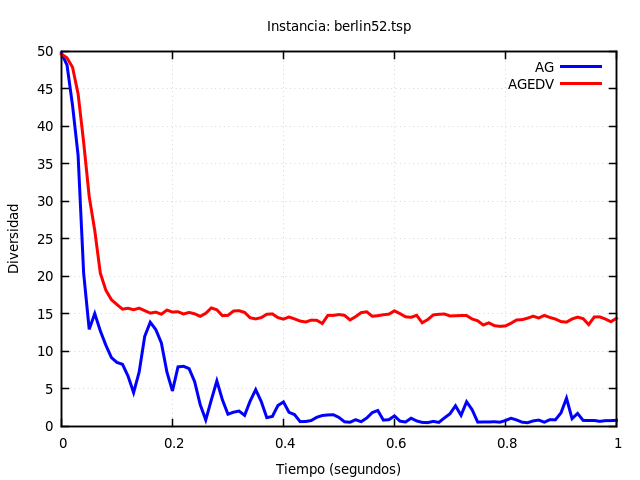
\includegraphics[width=7cm]{./Images/Diversity/AGEDV/png/berlin52.png}
			
			\column{.4\textwidth}
			
			\fontsize{9}{10}
			\selectfont
			\begin{center}
				\textbf{Diversidad en la población del AGEDV.}
			\end{center}			

			\kern -0.35cm

			\fontsize{8}{10}\selectfont
			\begin{itemize}
				\item Preservación de la diversidad mediante la {\color{red}diversificación voraz}.
				\item Uso productivo de la diversidad gracias a componentes específicas.

			\end{itemize}
			
		\end{columns}
		
		\kern 4mm
		\fontsize{6}{6}\selectfont

		\begin{tcolorbox}[colback=white,colframe=blue!30]
		\centering
		A. Herrera-Poyatos y F. Herrera, \textit{Algoritmo genético equilibrado con diversicación voraz}. Congreso Español
		de Metaheurísticas, Algoritmos Evolutivos y Bioinspirados – MAEB 2015, pp. 9-18, 2015.
		\end{tcolorbox}
			
	\end{frame}
}

{
	% Set the headline 
	\setbeamertemplate{headline}{
		\begin{beamercolorbox}[sep=10pt]{title} 
			\centering			
			\usebeamerfont{title} Motivación: Búsqueda de un algoritmo más eficaz.
	
			\kern 2mm
	
			Algoritmos Meméticos
		\end{beamercolorbox}
	}
	
	\begin{frame}{}
		
		% Font size
		\fontsize{9}{10}\selectfont
		
		\kern 5mm

		\centering
		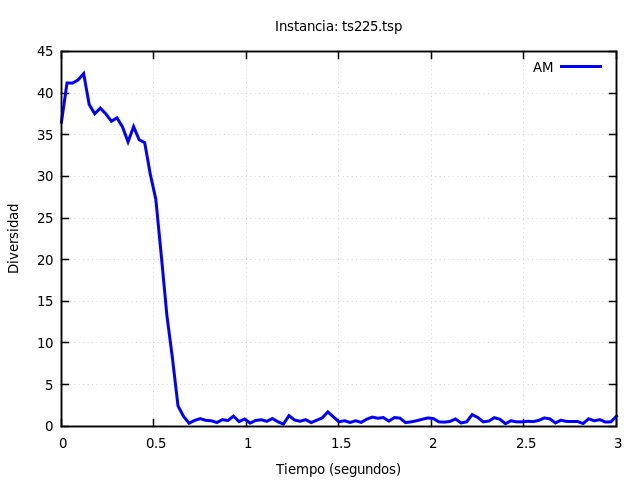
\includegraphics[width=7cm]{./Images/Diversity/AM/png/ts225.png}

		\kern 3mm
		
		\begin{tcolorbox}[colback=blue!5,colframe=blue!30]
			\centering
			\textbf{Problema de la diversidad de la población en algoritmos meméticos.}
		\end{tcolorbox}
		
	\end{frame}
}

{
	% Set the headline 
	\setbeamertemplate{headline}{
		\begin{beamercolorbox}[sep=10pt]{title} 
			\centering			
			\usebeamerfont{title} Objetivo: Búsqueda de un nuevo algoritmo memético
			
			\kern 2mm 

			con equilibrio entre diversidad y eficacia.
		\end{beamercolorbox}
	}
	
	\begin{frame}{}
		
		\kern 0.8cm
		\centering
		\begin{tikzpicture}[
			every node/.style={circle,inner sep=4pt, text width=2cm, align=center, node distance=1.5cm}]
				
			\node [fill=blue!20] (bl) {AGEDV};
			\node [fill=blue!60, above = of $(bl)$] (ag) {Algoritmos meméticos};
			\node [fill=blue!40, right= 2.5cm of {$(ag)!0.5!(bl)$}] (am) {		\fontsize{20}{10}\selectfont ?};
				
			\draw [->, >=stealth', line width=0.5mm] (bl) -- (am);
			\draw [->, >=stealth', line width=0.5mm] (ag) -- (am);
				
		\end{tikzpicture}		

		\kern 1.5mm

		\fontsize{12}{10}\selectfont

		\begin{tcolorbox}[colback=blue!5,colframe=blue!30]
			\centering
			\textbf{Algoritmo Memético Equilibrado con \\ Diversificación Voraz}
		\end{tcolorbox}
		
	\end{frame}
}